%input macros (i.e. write your own macros file called MacroFile1.tex)
%\newcommand{\PdfPsText}[2]{
  \ifpdf
     #1
  \else
     #2
  \fi
}

\newcommand{\IncludeGraphicsH}[3]{
  \PdfPsText{\includegraphics[height=#2]{#1}}{\includegraphics[bb = #3, height=#2]{#1}}
}

\newcommand{\IncludeGraphicsW}[3]{
  \PdfPsText{\includegraphics[width=#2]{#1}}{\includegraphics[bb = #3, width=#2]{#1}}
}

\newcommand{\InsertFig}[3]{
  \begin{figure}[!htbp]
    \begin{center}
      \leavevmode
      #1
      \caption{#2}
      \label{#3}
    \end{center}
  \end{figure}
}


%%% Local Variables: 
%%% mode: latex
%%% TeX-master: "~/Documents/LaTeX/CUEDThesisPSnPDF/thesis"
%%% End: 


 \documentclass[oneside,12pt]{Classes/CUEDthesisPSnPDF}

\usepackage{glossaries}

\makeglossaries

\newacronym{SNP}
{
    name=SNP,
    description={Single Nucleotide Polymorphism}
}

\ifpdf
    \pdfinfo { /Title  (CUED PhD and MPhil Thesis Classes)
               /Creator (TeX)
               /Producer (pdfTeX)
               /Author (Tommy Carstensen tc446@cam.ac.uk)
               /CreationDate (D:20140101000000)  %format D:YYYYMMDDhhmmss
               /ModDate (D:20141215000000)
               /Subject (Genetics)
               /Keywords (PhD, Thesis)}
    \pdfcatalog { /PageMode (/UseOutlines)
                  /OpenAction (fitbh)  }
\fi

\title{My PhD Thesis\\[1ex]
        in \LaTeX}

\ifpdf
  \author{\href{mailto:tc446@cam.ac.uk}{Tommy Carstensen}}
  \collegeordept{\href{http://www.phpc.cam.ac.uk/}{Department of Public Health and Primary Care}}
  \university{\href{http://www.cam.ac.uk}{University of Cambridge}}
% insert below the file name that contains the crest in-place of 'UnivShield'
  \crest{
\includegraphics[width=30mm]{UnivShield}}
\else
  \author{Tommy Carstensen}
  \collegeordept{Department of Public Health and Primary Care}
  \university{University of Cambridge}
% insert below the file name that contains the crest in-place of 'UnivShield'
  \crest{
\includegraphics[bb = 0 0 292 336, width=30mm]{UnivShield}}
\fi
%
% insert below the file name that contains the crest in-place of 'UnivShield'
% \crest{\IncludeGraphicsW{UnivShield}{40mm}{14 14 73 81}}
%
%\renewcommand{\submittedtext}{change the default text here if needed}
\degree{Doctor of Philosophy}
\degreedate{degreedate}

% turn of those nasty overfull and underfull hboxes
\hbadness=10000
\hfuzz=50pt

% Put all the style files you want in the directory StyleFiles and usepackage like this:
\usepackage{StyleFiles/watermark}

% Comment out the next line to get single spacing
\onehalfspacing

\begin{document}

%\language{english}

% A page with the abstract on including title and author etc may be
% required to be handed in separately. If this is not so, then comment
% the below 3 lines (between '\begin{abstractseparte}' and 
% 'end{abstractseparate}'), normally like a declaration ... needs some more
% work, mind as environment abstracts creates a new page!
% \begin{abstractseparate}
%   
% Thesis Abstract -----------------------------------------------------


%\begin{abstractslong}    %uncommenting this line, gives a different abstract heading
\begin{abstracts}        %this creates the heading for the abstract page

This is where you write your abstract ...


\end{abstracts}
%\end{abstractlongs}


% ----------------------------------------------------------------------


%%% Local Variables: 
%%% mode: latex
%%% TeX-master: "../thesis"
%%% End: 

% \end{abstractseparate}




% Using the watermark package which is in StyleFiles/
% and to remove DRAFT COPY ONLY appearing on the top of all pages comment out below line
%\watermark{DRAFT COPY ONLY}


\maketitle

%set the number of sectioning levels that get number and appear in the contents
\setcounter{secnumdepth}{3}
\setcounter{tocdepth}{3}

\frontmatter % book mode only
\pagenumbering{roman}
%% Thesis Dedictation ---------------------------------------------------

\begin{dedication} %this creates the heading for the dedication page

I would like to dedicate this thesis to ...

\end{dedication}

% ----------------------------------------------------------------------

%%% Local Variables: 
%%% mode: latex
%%% TeX-master: "../thesis"
%%% End: 

%% Thesis Acknowledgements ------------------------------------------------


%\begin{acknowledgementslong} %uncommenting this line, gives a different acknowledgements heading
\begin{acknowledgements}      %this creates the heading for the acknowlegments


And I would like to acknowledge ...


\end{acknowledgements}
%\end{acknowledgmentslong}

% ------------------------------------------------------------------------

%%% Local Variables: 
%%% mode: latex
%%% TeX-master: "../thesis"
%%% End: 

%
% Thesis Abstract -----------------------------------------------------


%\begin{abstractslong}    %uncommenting this line, gives a different abstract heading
\begin{abstracts}        %this creates the heading for the abstract page

This is where you write your abstract ...


\end{abstracts}
%\end{abstractlongs}


% ----------------------------------------------------------------------


%%% Local Variables: 
%%% mode: latex
%%% TeX-master: "../thesis"
%%% End: 


\tableofcontents
\listoffigures
\listoftables
\printnomenclature  %% Print the nomenclature
\printglossary[type=\acronymtype]
\addcontentsline{toc}{chapter}{Nomenclature}

\mainmatter % book mode only
%%% Thesis Introduction --------------------------------------------------
\chapter{Introduction}
\ifpdf
    \graphicspath{{Introduction/IntroductionFigs/PNG/}{Introduction/IntroductionFigs/PDF/}{Introduction/IntroductionFigs/}}
\else
    \graphicspath{{Introduction/IntroductionFigs/EPS/}{Introduction/IntroductionFigs/}}
\fi

We study genetics in Africa for several reasons. To illuminate recent human evolution and demographic history. To study the genetics of susceptibility to communicable and non-communicable diseases, which are widespread in Africa.
genetic variation greater in Africa\cite{RosenbergScience2002}

%%% ----------------------------------------------------------------------


%%% Local Variables: 
%%% mode: latex
%%% TeX-master: "../thesis"
%%% End: 

% \pagebreak[4]
% \hspace*{1cm}
% \pagebreak[4]
% \hspace*{1cm}
% \pagebreak[4]

\chapter{Cost Effective Study Design in an African Population}
\ifpdf
    \graphicspath{{Chapter1/Chapter1Figs/PNG/}{Chapter1/Chapter1Figs/PDF/}{Chapter1/Chapter1Figs/}}
\else
    \graphicspath{{Chapter1/Chapter1Figs/EPS/}{Chapter1/Chapter1Figs/}}
\fi

%A \acrlong{SNP} is abbreviated abbreviated \acrshort{SNP}.
A \gls{SNP} is a \Gls{SNP} is a \GLS{SNP}. Testing glossary.

\section{Introduction}
\section{Data Description}
Omni/HiSeq Sample count table. Omni/HiSeq SNP count table. Sample coverage table.
\section{Methods}
\subsection{SNP Chip Array QC}
\subsection{Sequencing}
The ability to sequence depends on the sequence content and the ability to map depends on the uniqueness of the sequence and the presence and length of indels.
\subsection{Downsampling}
GATK PrintReads\cite{DePristo2011}
\subsection{BAM pre-processing}
We carry out base quality score recalibration. Base quality doesn't have any impact on indel realignment, so it wouldn't make a difference. But having reads realigned properly improves the base recalibration model because it reduces the number of artifactual SNPs.
We mark duplicates for exclusion with Picard, because sequencing errors are otherwise propagated in duplicates leading to false positive variant calls.
\subsubsection{Realignment around INDELs}
Improves accuracy of downstream processing steps. Avoid mappers mis-aligning with mismatches. Regions that need to be realigned are identified with GATK RealignerTargetCreater and the actual realignment is performed with GATK IndelRealigner.
%Ask Martin if he uses the -known flag, which is accurate for ~90-95% of indels. Check if info in BAM header.
%Recommendations here: https://www.broadinstitute.org/gatk/guide/article?id=1247
\subsection{Variant Calling}
Also include samtools, FreeBayes and Platypus.
Remember that HC does INDEL realignment on the fly...
Minimum read mapping quality required to consider a read for analysis with the HaplotypeCaller (HCMappingQualityFilter) (--min_mapping_quality_score 20)
HC DuplicateReadFilter
Target coverage threshold for downsampling to coverage HC --downsampling_type BY_SAMPLE --downsample_to_coverage 250
Minimum base quality required to consider a base for calling --min_base_quality_score 10 (UG17)
The minimum phred-scaled confidence threshold at which variants should be called --standard_min_confidence_threshold_for_calling
The minimum phred-scaled confidence threshold at which variants should be emitted (and filtered with LowQual if less than the calling threshold) --standard_min_confidence_threshold_for_emitting
HC only maxNumHaplotypesInPopulation 128
max_alternate_alleles 6
%INDELs, especially those disrupting protein-coding regions of the genome, have been strongly associated with human diseases.
%http://www.ncbi.nlm.nih.gov/clinvar?term=human%5Borgn%5D
\subsection{Variant Filtering}
VQSLOD is the log odds ratio of being a true variant versus being false.
\subsection{Genotype refinement}
1000G because small sample size!
\subsection{WGS QC}
\section{Results}
\subsection{Comparison of variant calling and refinement methods}
\subsection{Comparison of variant calling software}
\subsection{Comparison of refinement software and reference panels}
\subsection{Statistics after downsampling}
Lots of table and figures. Copy/Paste from Word.
\subsection{Apparent sample size}
\section{Discussion}
\section{Conclusions}

%\section{First Paragraph}
And now I begin my first chapter here ...

Here is an equation\footnote{the notation is explained in the nomenclature section :-)}:
\begin{eqnarray}
CIF: \hspace*{5mm}F_0^j(a) &=& \frac{1}{2\pi \iota} \oint_{\gamma} \frac{F_0^j(z)}{z - a} dz
\end{eqnarray}
\nomenclature[zcif]{$CIF$}{Cauchy's Integral Formula}                                % first letter Z is for Acronyms 
\nomenclature[aF]{$F$}{complex function}                                                   % first letter A is for Roman symbols
\nomenclature[gp]{$\pi$}{ $\simeq 3.14\ldots$}                                             % first letter G is for Greek Symbols
\nomenclature[gi]{$\iota$}{unit imaginary number $\sqrt{-1}$}                      % first letter G is for Greek Symbols
\nomenclature[gg]{$\gamma$}{a simply closed curve on a complex plane}  % first letter G is for Greek Symbols
\nomenclature[xi]{$\oint_\gamma$}{integration around a curve $\gamma$} % first letter X is for Other Symbols
\nomenclature[rj]{$j$}{superscript index}                                                       % first letter R is for superscripts
\nomenclature[s0]{$0$}{subscript index}                                                        % first letter S is for subscripts

%\section{Second Paragraph}
and here I write more ...\cite{texbook}

%\subsection{sub first paragraph}
... and some more ...

Now I would like to cite the following: \cite{latex} and \cite{texbook}
and \cite{Rud73}.

I would also like to include a picture ...

\begin{figure}[!htbp]
  \begin{center}
    \leavevmode
    \ifpdf
      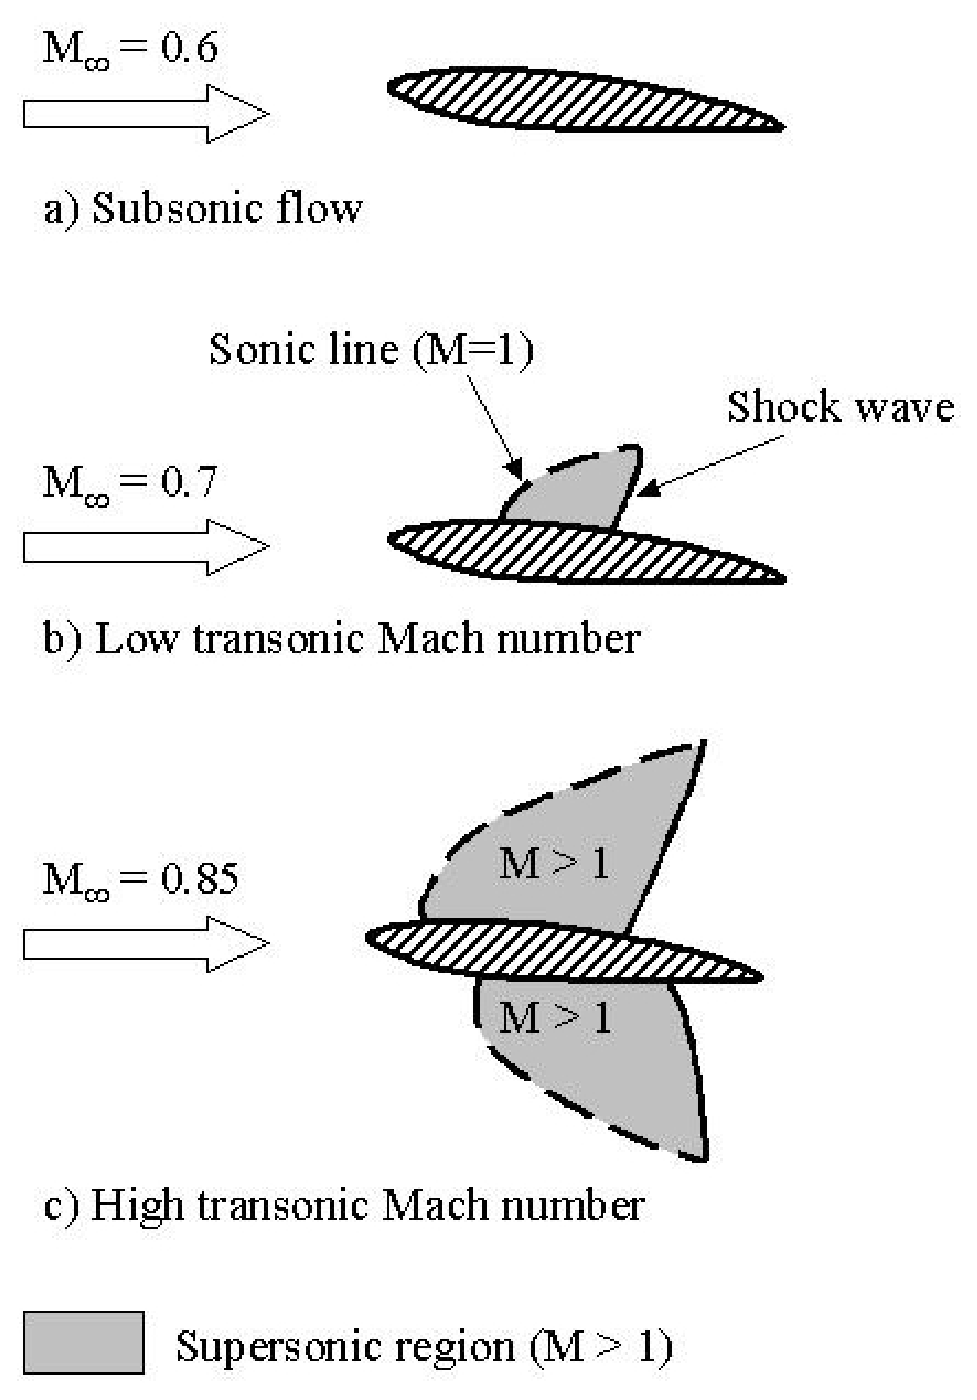
\includegraphics[height=6in]{aflow}
    \else
      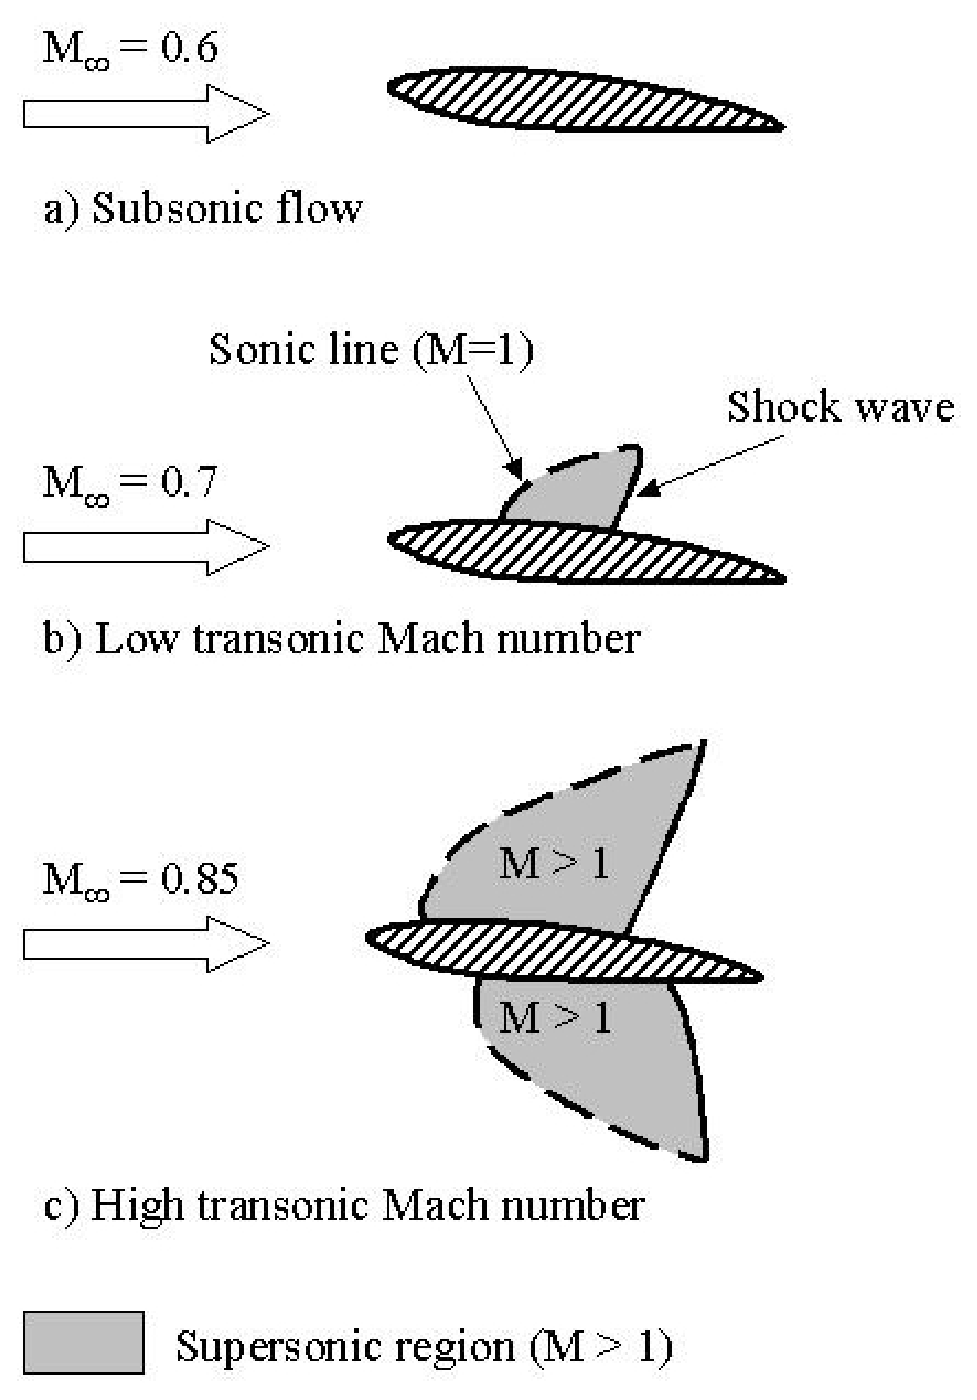
\includegraphics[bb = 92 86 545 742, height=6in]{aflow}
    \fi
    \caption{Airfoil Picture}
    \label{FigAir}
  \end{center}
\end{figure}

% above code has been macro-fied in Classes/MacroFile.tex file
%\InsertFig{\IncludeGraphicsH{aflow}{6in}{92 86 545 742}}{Airfoil Picture}{FigAir}

So as we have now labelled it we can reference it, like so (\ref{FigAir}) and it
is on Page \pageref{FigAir}. And as we can see, it is a very nice picture and we
can talk about it all we want and when we are tired we can move on to the next
chapter ...

I would also like to add an extra bookmark in acroread like so ...
\ifpdf
  \pdfbookmark[2]{bookmark text is here}{And this is what I want bookmarked}
\fi
% ------------------------------------------------------------------------


%%% Local Variables: 
%%% mode: latex
%%% TeX-master: "../thesis"
%%% End: 

\chapter{Generation of a Reference Panel for the African Continent}
\ifpdf
    \graphicspath{{Chapter2/Chapter2Figs/PNG/}{Chapter2/Chapter2Figs/PDF/}{Chapter2/Chapter2Figs/}}
\else
    \graphicspath{{Chapter2/Chapter2Figs/EPS/}{Chapter2/Chapter2Figs/}}
\fi

\section{Introduction}
\section{Data Description}
Reference tables in chapter1.
\section{Methods}
\subsection{SNP Chip Array QC and post-processing}
\subsection{Phasing of Refined Genotypes}
\subsection{Generation of a Merged Reference Panel}
\section{Results}
\subsection{SNP Similarities and Differences between Populations}
SNP Venn Diagrams
\subsection{SNP Chip Array and Sequence Comparative Statistics for Each Population}
\subsection{Improved Imputation Accuracy with African Reference Panel}
\subsection{Comparison of SNP Chip Arrays}
Comparison of YRI, LWK, MSL, xxx, xxx, Uganda, Zulu, Ethiopia capture.
\section{Discussion}
\section{Conclusions}

%\section{First Section}
\markboth{\MakeUppercase{\thechapter. My Second Chapter }}
And now I begin my second chapter here ...

%\section{Second Section}
\markboth{\MakeUppercase{\thechapter. My Second Chapter }}
and here I write more ...

% ------------------------------------------------------------------------

%%% Local Variables: 
%%% mode: latex
%%% TeX-master: "../thesis"
%%% End: 

\chapter{Design of a SNP Genotyping Array Specific to the African Continent}
\ifpdf
    \graphicspath{{Chapter3/Chapter3Figs/PNG/}{Chapter3/Chapter3Figs/PDF/}{Chapter3/Chapter3Figs/}}
\else
    \graphicspath{{Chapter3/Chapter3Figs/EPS/}{Chapter3/Chapter3Figs/}}
\fi

\section{Introduction}
Text
\section{Data description}
\section{Methods}
Text
\subsection{Selection of tag SNPs}
\subsubsection{Greedy tag SNP Selection Algorithm}
\subsubsection{Imputation with IMPUTE2}
\section{Results}
\subsection{Comparison of RagTagger with Existing Methods}
\subsection{Comparison of the Simple Greedy Algorithm and the Hybrid Algorithm}
\section{Discussion}
\section{Conclusions}

%\section{First Section of the Third Chapter}
\markboth{\MakeUppercase{\thechapter. My Third Chapter }}{\thechapter. My Third Chapter}
And now I begin my third chapter here ...

\markboth{\MakeUppercase{\thechapter. My Third Chapter }}{\thechapter. My Third Chapter}
and here I write more ...

% ------------------------------------------------------------------------


%%% Local Variables: 
%%% mode: latex
%%% TeX-master: "../thesis"
%%% End: 

%\chapter{ug2g}
\ifpdf
    \graphicspath{{Chapter3/Chapter3Figs/PNG/}{Chapter3/Chapter3Figs/PDF/}{Chapter3/Chapter3Figs/}}
\else
    \graphicspath{{Chapter3/Chapter3Figs/EPS/}{Chapter3/Chapter3Figs/}}
\fi

\Section

%\section{First Section of the Third Chapter}
\markboth{\MakeUppercase{\thechapter. My Third Chapter }}{\thechapter. My Third Chapter}
And now I begin my third chapter here ...

\markboth{\MakeUppercase{\thechapter. My Third Chapter }}{\thechapter. My Third Chapter}
and here I write more ...

% ------------------------------------------------------------------------


%%% Local Variables: 
%%% mode: latex
%%% TeX-master: "../thesis"
%%% End: 

\def\baselinestretch{1}
\chapter{My Conclusions ...}
\ifpdf
    \graphicspath{{Conclusions/ConclusionsFigs/PNG/}{Conclusions/ConclusionsFigs/PDF/}{Conclusions/ConclusionsFigs/}}
\else
    \graphicspath{{Conclusions/ConclusionsFigs/EPS/}{Conclusions/ConclusionsFigs/}}
\fi

\def\baselinestretch{1.66}

Here I put my conclusions ...

%%% ----------------------------------------------------------------------

% ------------------------------------------------------------------------

%%% Local Variables: 
%%% mode: latex
%%% TeX-master: "../thesis"
%%% End: 


\backmatter % book mode only
\appendix
\chapter{Appdx A}

and here I put a bit of postamble ...

% ------------------------------------------------------------------------

%%% Local Variables: 
%%% mode: latex
%%% TeX-master: "../thesis"
%%% End: 

\chapter{Appdx B}

and here I put some more postamble ...

% ------------------------------------------------------------------------

%%% Local Variables: 
%%% mode: latex
%%% TeX-master: "../thesis"
%%% End: 


\bibliographystyle{plainnat}
%\bibliographystyle{Classes/CUEDbiblio}
%\bibliographystyle{Classes/jmb}
%\bibliographystyle{Classes/jmb} % bibliography style
\renewcommand{\bibname}{References} % changes default name Bibliography to References
\bibliography{References/references} % References file

\end{document}
